\documentclass{article}
\usepackage{graphicx} % Required for inserting images
\usepackage{algorithm}
\usepackage{algpseudocode}
\usepackage{float}       % For [H] placement
\usepackage[a4paper, margin=0.5in]{geometry}
\usepackage[font=scriptsize,labelfont=bf]{caption}
\captionsetup[figure]{justification=centering, font=small}
\usepackage{hyperref}
\hypersetup{
  colorlinks   = true,
  linkcolor    = blue,
  citecolor   = red
}

\title{Mesh Adapt Pseudo Code}
\author{}
\date{}

\begin{document}

\maketitle

\section{Algorithms}


\begin{algorithm}
\caption{Adapt Top Level}
\begin{algorithmic}[1]
    \State $Input:$ desired mesh size field
    \State $MetricLength=$ loop over all edges to find the longest edge in the metric space
    \State $NumIterations=$ $log_2(MetricLength)+1$ rounded up
    \For{$i = 0$ to $NumIterations$}
        \State coarsen() \Comment {remove short edges from input mesh and created during refinement and snapping}
        \State refine() \Comment {split long edges to reach desired size}
        \State snap() \Comment {move vertices created in refine step to model boundary}
    \EndFor
    \State fixShape() \Comment {remove or improve low quality tetrahedrons}
\end{algorithmic}
\end{algorithm}


\textbf{Coarsen:} Remove edges below minimum edge length in metric space using Algorithm 2. This is first to reduce the peak memory use by reducing the size of the mesh. It must be re-run because refinement and snapping can create additional short edges.

\textbf{Refine:} Loop through all edges and flag edges above the maximum edge length in the metric space. Split all these edges and their adjacent elements once. This is done in steps because it results in higher quality elements.

\textbf{Snap:} Move new vertices created from refinement to the model boundary using Algorithm 3.

\textbf{FixShape:} loop through all the tetrahedrons to determine which are below the desired quality in the metric space and eliminate them using Algorithm 4. This is done at the end to clean up any poor quality tetrahedrons that could have been created by the user or previous steps.

\begin{figure}[H]
    \centering
    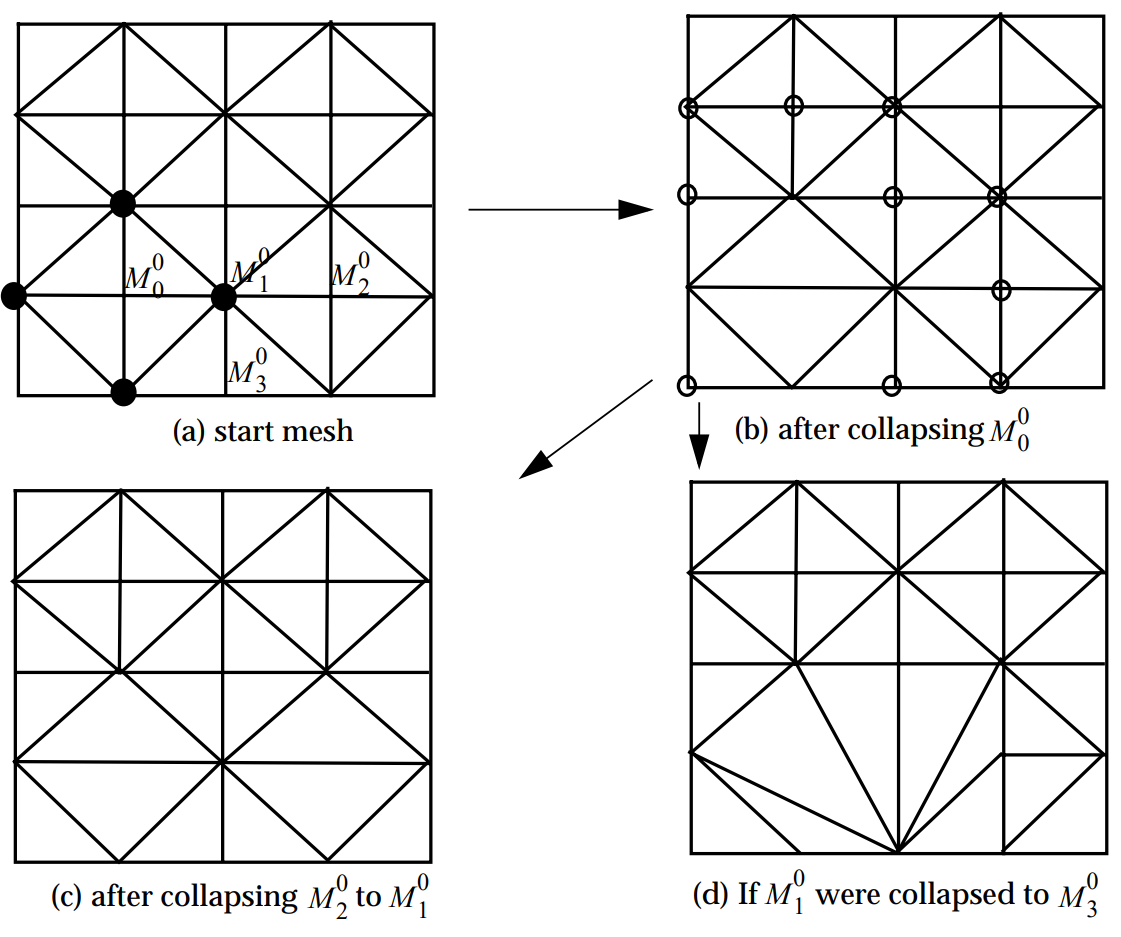
\includegraphics[width=0.5\linewidth]{adapt_coarsen_order.png}
    \caption{Importance of collapsing every other vertex. Reproduced from Li's Thesis}
    \label{coarsenOrder}
\end{figure}

\textbf{Coarsen:} The following algorithm collects a list of vertices adjacent to a short edge and then collapse those short edges while avoiding a collapse of two adjacent vertices in a row. \autoref{coarsenOrder} shows the issue with collapsing two adjacent vertices. Collapsing the doted vertices in example (a) is bad because it causes the edges to be pulled in one direction as shown in example (d). Instead collapsing one of the circled vertices in example (b) results in a higher quality mesh line in example (c).  
    
Lines 1-11, obtain a list of vertices adjacent to short edges and the flag is being used to avoid duplicates in the list.

Lines 12-13, flag indicate whether more collapses need to be tried. This flag is changed in line 26 because a successful collapse creates more space for collapses to succeed and it also creates an dependent set that needs to be tried in future loops.

Lines 14-18, obtain a vertex from the list and checking if its available for collapse using a flags. There are multiple reason a vertex may or may not be available for collapse.

Line 18, the vertex is being flagged to prevent it from being checked again.

Line 24, the flag is removed because a collapse can increase the changes of an adjacent collapse succeeding, so those vertices need to be processed again.

Line 25, adjacent vertices are marked as a dependent set to prevent them from collapsing until the independent set is finished.

Lines 19-23, attempt several collapses starting with the shortest edge first. The shortest edge first to prioritize getting rid of the shortest edges and they also result in the smallest change to the resulting mesh meaning that they are more likely to succeed and creates higher quality elements. A collapse might fail if it causes adjacent element to become invalid because of improper classification or inverted or negative volume.

\begin{algorithm}[H]
\caption{Coarsen}
\begin{algorithmic}[1]
    \ForAll {edges}
        \If {edge length in metric space $<$ minimum edge length}
            \ForAll {vertices $M^0_i$ in edge} \Comment {edges have 2 vertices}
                \If {$M^0_i$ not flagged} \Comment {flag indicates if $M^0_i$ has been added to list}
                    \State add $M^0_i$ to the process list
                \EndIf
                \State flag $M^0_i$ as checked \Comment {flag to ensure $M^0_i$ added to list once}
            \EndFor
        \EndIf
    \EndFor
    \State remove the flag from all vertices
    \While {$done == false$} \Comment{flag indicates whether more independent sets are necessary}
        \State $done = true$
        \While {there there is unchecked vertex $M^0_i$}
            \If {$M^0_i$ is $checked$ or is $dependent$} \Comment {flags indicates if $M^0_i$ can be collapsed}
                \State \textbf{continue}
            \EndIf
            \State flag vertex $M^0_i$ as $checked$ \Comment {ensure $M^0_i$ not processed again unless cavity changes}
            \State collect a list of adjacent edges $L$
            \State sort $L$ by edge length in metric space
            \ForAll {edges $L_e$ in $L$ starting with the shortest}
                \State evaluate a collapse on $L_e$ with $M^0_i$ removed
                \If {collapse passes checks for classification, geometry and quality}
                    \State remove $checked$ flag from adjacent vertices 
                    \State flag adjacent vertices as $dependent$
                    \State $done = false$
                    \State rebuild the cavity
                    \State \textbf{break} \Comment {stop evaluating and skip $M^0_{i+1}$}
                \EndIf
            \EndFor
        \EndWhile
        \State clear dependent flags from mesh
    \EndWhile
\end{algorithmic}
\end{algorithm}

\textbf{Refine:} The following algorithm collects a list of edges that need to be split into smaller edges and then splits those edges and create new adjacent elements and transfer all of the data to the new elements. 

Lines 1-5, find edges that are longer than the max edge length and flag them. The flag is used to avoid recomputing the expensive metric length computation.

Lines 6-20, count the number of edges, faces, and regions that need to be split while using a flag to avoid double counting.

Line 21, create a list with space for each entity counted in lines 6-20. This list is used to keep a pointer for cleanup of data after the old entities are split. 

Lines 22-38, populate the $Old$ list with the counted entities using the flags again to avoid adding the same entity twice. 

Line 39, create a list to store the new entities created. This list is the same size as the Old list except it contains a list of entities for each old entity. This list is used for transferring data to all of the new entities as a group after refinement is done. 

Lines 40-48, iterate through the old elements, split them, transfer some of the information and then add the new elements to the list. 

Lines 49-51, transfer the rest of the necessary data to the new elements. 

Lines 52-54, destroy the allocation for the old elements. 

Line 55, destroy the list pointing to the Old and New elements.


\begin{algorithm}[H]
\caption{Refine}
\begin{algorithmic}[1]
\ForAll {edges $E_i$ in mesh}
    \If {$E_i$ length in metric space $>$ maximum edge length}
        \State flag $E_i$ with split flag
    \EndIf
\EndFor
\ForAll {edges $E_i$ in mesh} \Comment {flag and count upward elements}
    \If {$E_i$ has split flag}
        \State add $E_i$ to count
        \ForAll {faces $F_i$ adjacent to $E_i$}
            \If {$F_i$ does not have split flag} \Comment {used to prevent recounting}
                \State flag $F_i$ with split flag and add it to count
                \ForAll {regions $R_i$ adjacent to $F_i$}
                    \If {$R_i$ does not have split flag}
                        \State flag $R_i$ with split flag and add it to count \Comment {used to prevent recounting}
                    \EndIf
                \EndFor
            \EndIf
        \EndFor
    \EndIf
\EndFor
\State allocate 2D array $Old$ with space for each flagged edge, face, and region
\ForAll {edges $E_i$ in mesh} \Comment {add flagged edges, faces and regions to newly allocated array}
    \If {$E_i$ has split flag}
        \State $Old_{i} = E_i$ 
        \ForAll {faces $F_j$ adjacent to $E_i$}
            \If {$F_j$ has split flag} \Comment {used to prevent re-adding}
                \State $Old_{j} = F_j$
                \State clear split flag
                \ForAll {regions $R_k$ adjacent to $F_j$} \Comment {used to prevent re-adding}
                    \If {$R_k$ has split flag}
                        \State $Old_{k} = R_k$
                        \State clear split flag from $R_k$
                    \EndIf
                \EndFor
            \EndIf
        \EndFor
    \EndIf
\EndFor
\State allocate 2D array $New$ with same size as $Old$ which contains edge, face, and region
\ForAll {elements $Old_i$ in $Old$}
    \If {$Old_i$ is an edge}
        \State create vertex
        \State transfer parametric coordinates and interpolate
        \State tag vertex to snap
    \Else
        \State find newly created downward elements $D$ in mesh
        \State build new element connected to $D$
    \EndIf
    \State add new elements to $New_i$
\EndFor
\ForAll {elements $New_i$ in $New$}
    \State transfer coordinate, solution transfer and size field data from $Old_i$ to $New_i$
\EndFor
\ForAll {elements $Old_i$ in $Old$}
    \State destroy $Old_i$
\EndFor
\State de-allocate $Old$ and $New$

\end{algorithmic}
\end{algorithm}


\begin{figure}[H]
    \centering
    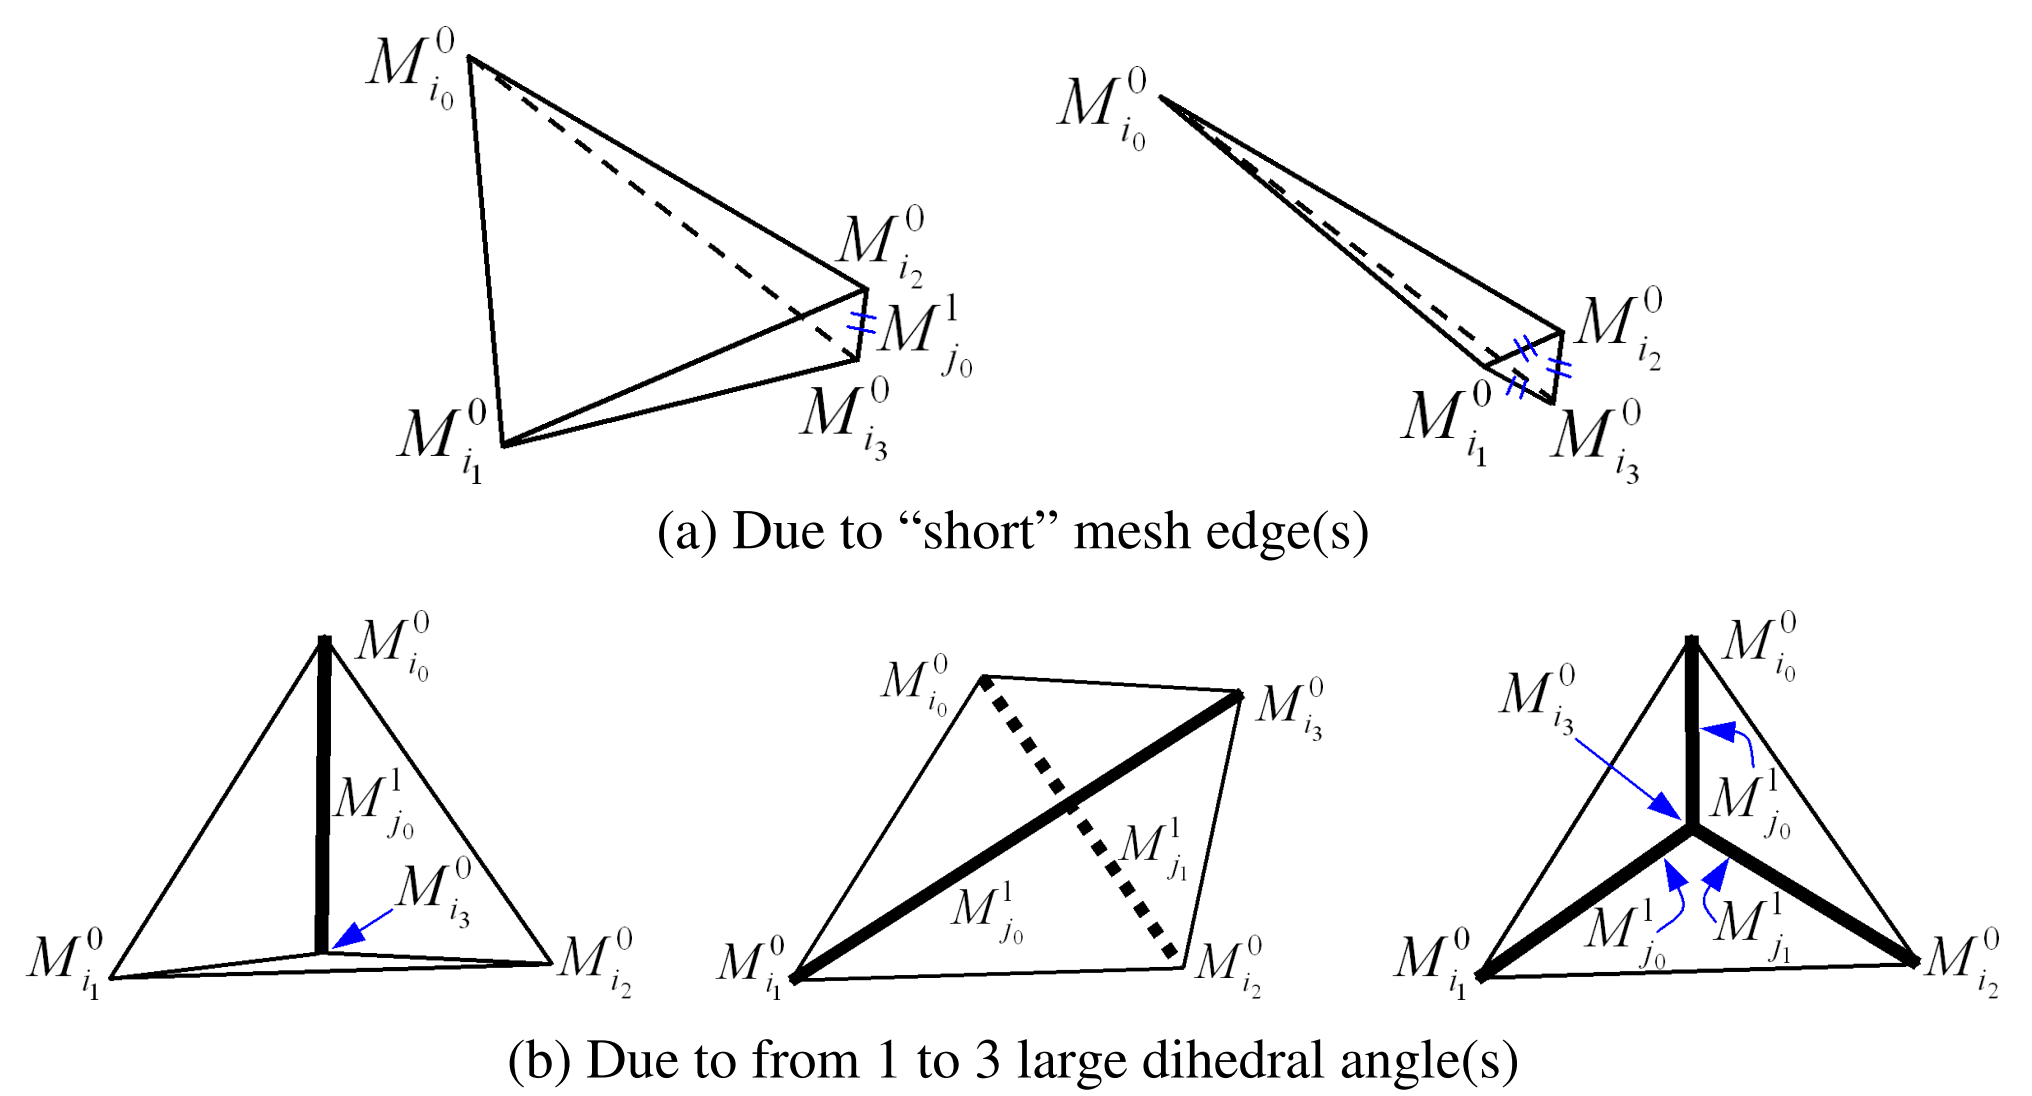
\includegraphics[width=0.7\linewidth]{adapt_tet_types.png}
    \caption{Types of low quality tetrahedron \\
    Reproduced from Wan, J., "An automated adaptive procedure for 3D metal forming simulations", Ph.D. Thesis, Rensselaer Polytechnic Institute, Troy, NY 12180 (2006)}
    \label{tetTypes}
\end{figure}

\autoref{tetTypes} shows multiple types of tetrahedron that are not desirable. Section (a) includes two shapes that are undesirable due to having one or three short edges. Section b includes three shapes that are undesirable due to their low quality. Low quality shapes fall along a continuum of shapes between one, two, or three large dihedral angles. These shapes and how to remove or improve them shall be referenced in the following algorithms. Each operator checks that the operator should pass geometric, classification and quality checks. Each shape has multiple local operations that can be used to improve the quality, and different operations are considered in the order that is most likely to succeed. After a successful operation will stop execution and continue to the next tetrahedron.

\textbf{Fix Shape:} The following algorithm takes a mesh with low quality tetrahedrons and either find the best method to remove them or to improve their quality.

Lines 1-6, measures the quality of the tetrahedron and counting and flagging them. The count tracks if at improving the quality of the shapes. This is necessary because several operators (like split-collapse) can remove a low quality shape and create more than one slightly better low quality shape. So the count ensure that the algorithm doesn't get stuck creating more and more bad shapes.

Lines 7-11, start with collapsing short edges because this operator is the most likely to succeed.

Lines 8-16, attempt some collapses that result in the short edge merging into a larger edge.

Lines 17-37, determine the type of low quality tetrahedrons and then evaluate operations in an order that optimizes for quality and runtime. After the first operation succeeds the rest don't need to be evaluated. Collapse operations first because they always decrease the number of elements. Then compound operators second because while they are more likely to succeed, there is a high chance that they create low quality elements. Reposition last because while it is almost guaranteed to improve the shape, it also has the slowest runtime.


\begin{figure}[H]
    \centering
    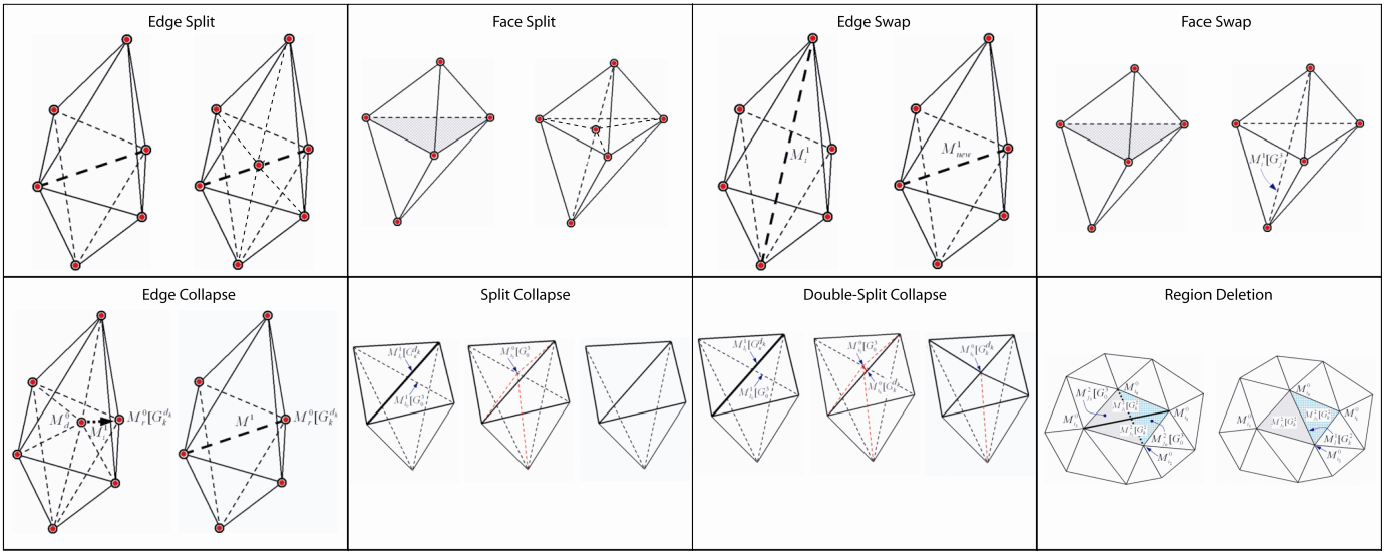
\includegraphics[width=1.0\linewidth]{adapt_local_operations.png}
    \caption{Local mesh modification operations. Reproduced from SCOREC papers.}
    \label{meshOperations}
\end{figure}


\begin{algorithm}[H]
\caption{Fix Element Shapes}
\begin{algorithmic}[1]
\ForAll {tetrahedrons}
    \If {quality of tetrahedron $<$ minimum quality}
        \State count and flag tetrahedron to be processed
    \EndIf
\EndFor
\While {the number of low quality tetrahedron decreases} \Comment {first successful evaluate skips to next tetrahedron}
    \ForAll {edges in tetrahedron}
        \If {length of edge $<$ minimum length} \Comment{this value is cached}
            \If {collapse short edge}
                \State go to next tetrahedron
            \EndIf
        \EndIf
    \EndFor
    \ForAll {edges in tetrahedron}
        \If {length of edge $M^1_i$ $<$ minimum length} \Comment{this value is cached}
            \If {collapsing adjacent edges that result in $M^1_i$ becoming longer}
                \State go to next tetrahedron
            \EndIf
        \EndIf
    \EndFor
    \If {\textbf{one large dihedral angle}}
        \If {region-collapse if the tetrahedron is on the surface \\
        \hspace{.93cm} \textbf{or} edge-swap on the longest edge in the low quality triangle \\
        \hspace{.93cm} \textbf{or} split-collapse on the longest edge in the low quality triangle \\
        \hspace{.93cm} \textbf{or} edge-collapse on any edge in the low quality triangle besides the longest edge \\
        \hspace{.93cm} \textbf{or} reposition tetrahedron vertices to improve quality}
            \State go to next tetrahedron
        \EndIf
    \EndIf
    \If {\textbf{two large dihedral angles}}
        \If {evaluate region-collapse if the tetrahedron is on the surface \\
        \hspace{.93cm} \textbf{or} edge-swap on $M^{1}_{j_0}$ or $M^{1}_{j_1}$ \\
        \hspace{.93cm} \textbf{or} split-collapse on $M^{1}_{j_0}$ or $M^{1}_{j_1}$ \\
        \hspace{.93cm} \textbf{or} double-split-collapse on $M^{1}_{j_0}$ and $M^{1}_{j_1}$ \\
        \hspace{.93cm} \textbf{or} reposition tetrahedron vertices to improve quality}
            \State go to next tetrahedron
        \EndIf
    \ElsIf {\textbf{three large dihedral angles}}
        \If {edge-collapse on $M^{1}_{j_0}$, $M^{1}_{j_1}$, or $M^{1}_{j_2}$ with $M^{0}_{i_3}$ deleted \\
        \hspace{.93cm} \textbf{or} edge-swap on any edge bounding triangle made by $M^{0}_{i_0}$, $M^{0}_{i_1}$, and $M^{0}_{i_2}$ \\
        \hspace{.93cm} \textbf{or} face-swap on the triangle made by $M^{0}_{i_0}$, $M^{0}_{i_1}$, $M^{0}_{i_2}$ \\
        \hspace{.93cm} \textbf{or} split-collapse on the triangle made by $M^{0}_{i_0}$, $M^{0}_{i_1}$, $M^{0}_{i_2}$ with $M^{0}_{i_3}$ deleted \\
        \hspace{.93cm} \textbf{or} face-split-collapse on the triangle made by $M^{0}_{i_0}$, $M^{0}_{i_1}$, $M^{0}_{i_2}$ with $M^{0}_{i_3}$ deleted \\
        \hspace{.93cm} \textbf{or} reposition vertex $M^{0}_{i_3}$ to improve quality}
            \State go to next tetrahedron
        \EndIf
    \EndIf
\EndWhile

\end{algorithmic}
\end{algorithm}


\begin{figure}[H]
    \centering
    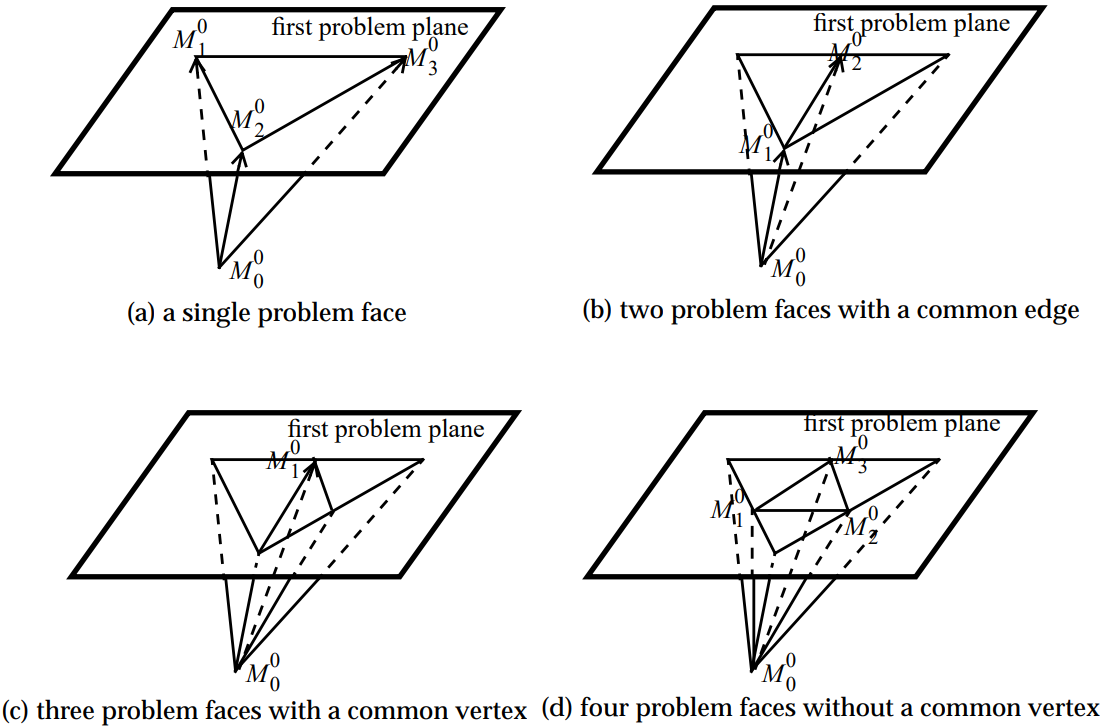
\includegraphics[width=0.8\linewidth]{adapt_common_edges.png}
    \caption{Types of common collapses. Reproduced from Li's Thesis}
    \label{commonCollapses}
\end{figure}

\textbf{Snapping:} Is a procedure where newly created vertices are relocated to the model boundary. Part of the algorithm is similar to fix shape, but with the direction of the operations restricted towards the model boundary.

Lines 1-7, flag all of the vertices that need to be snapped.

Lines 8-14, try to move the vertex directly to the model boundary. Most of the time this works and then it exits in line 13. Otherwise it reverts to the original state in line 11.

Lines 15-24, collect the first problem plane. This encompasses the entities that need to be changed before progress can be made towards the target. As shown in \autoref{commonCollapses} it can have one or multiple tetrahedron.

Lines 25-32, collect the common edges of the tetrahedron in the first problem plane. \autoref{commonCollapses}, shows the ideal way to reach the first problem plane is to collapse one of these edges. In example (a) any of the edges can be collapsed. In example (b) only two of the edges can be collapse with out creating invalid elements. In example (c) only one edge can be collapse. In example (d), none of the edges can be collapse.

Line 33, attempt to collapse one of the common edges.

Line 34, attempt to reduce one of the more complicated cases (b, c, d) into one of the simpler cases by collapsing shared edges of the first problem plane.

Line 35, evaluate adjacent collapses that might reduce the complexity of the first problem plane and still make some progress towards the first problem plane.

Lines 36-49, are a subset of fix shape, except only operations that make progress towards the first problem plane are considered.


\begin{algorithm}[H]
\caption{Snapping}
\begin{algorithmic}[1]
    \State \textbf{Input:} mesh with flagged new vertices on model boundary
    \While {there are any vertices flagged to snap}
        \State move the current vertex $M^0_i$ to the model boundary \Comment {attempt simple movement first}
        \If {any adjacent elements inverted}
            \State move $M^0_i$ to original position
        \Else
            \State remove the flag to snap from $M^0_i$ then \textbf{continue}
        \EndIf
        \ForAll {invalid adjacent tetrahedron $M^3_i$} \Comment {find the first problem plane}
            \State $ray = $ draw a ray from the start position to the target position
            \State $M^1_i =$ the face opposite to $M^0_i$ in $M^3_i$
            \State $distance = $ distance to intersection of the ray and $M^1_i$ on the infinite plane
            \If {distance $<$ minimum distance}
                \State list FPP = $M^3_i$
            \ElsIf {distance == minimum distance}
                \State add $M^3_i$ to the FPP list
            \EndIf
        \EndFor
        \ForAll {edges $M^1_i$ in FPP} \Comment {find common edges}
            \ForAll {tetrahedrons $M^3_j$ in FPP}
                \State find if $M^1_i$ in $M^3_j$
            \EndFor
            \If {$M^1_i$ in every tetrahedron}
                \State add $M^1_i$ to the common edge list
            \EndIf
        \EndFor
        \If {collapse common edges that move towards FPP with $M^0_i$ preserved \\
        \hspace{.4cm} \textbf{or} collapse edges on FPP that increase common edges \\
        \hspace{.4cm} \textbf{or} collapse common edges with $M^0_i$ preserved}
            \State go to $M^0_{i+1}$
        \EndIf
        \If {\textbf{one large dihedral angle}}
            \If {swap the longest edge \\
            \hspace{.93cm} \textbf{or} split-collapse on the longest edge}
                \State go to $M^0_{i+1}$
            \EndIf
        \EndIf
        \If {\textbf{two large dihedral angles}}
            \If {swap either $M^1_{j0}$ or $M^1_{j1}$ \\
            \hspace{.93cm} \textbf{or} split-collapse on either $M^1_{j0}$ or $M^1_{j1}$ \\
            \hspace{.93cm} \textbf{or} double-split-collapse on both $M^1_{j0}$ and $M^1_{j1}$}
                \State go to $M^0_{i+1}$
            \EndIf
        \ElsIf {\textbf{three large dihedral angles}}
            \If {swap any edge in face made by $M^{0}_{i_0}$, $M^{0}_{i_1}$, and $M^{0}_{i_2}$ \\
            \hspace{.93cm} \textbf{or} swap the problem face made by $M^{0}_{i_0}$, $M^{0}_{i_1}$, and $M^{0}_{i_2}$ \\
            \hspace{.93cm} \textbf{or} split-collapse on any edge in face made by $M^{0}_{i_0}$, $M^{0}_{i_1}$, and $M^{0}_{i_2}$}
                \State go to $M^0_{i+1}$
            \EndIf
        \EndIf
    \EndWhile
\end{algorithmic}
\end{algorithm}

\textbf{Future Work}

\begin{itemize}
    \item \textbf{Collapse-Swap:} This algorithm will swap invalid edges created a by a collapse in order to make the collapse succeed. This has the potential of improving runtime since not as many collapses have to be tested. In our current algorithm we have to test every short edge adjacent to a vertex, but in Li's algorithm he only has to test the shortest edge. In addition, collapsing the shortest edge generally results in better quality meshes since collapsing the shortest edge will result in the smallest change to the mesh.
    \item \textbf{Vertex Reposition:} This addition to the algorithm will improve edge lengths. As described in Li's algorithm, when a collapse creates an edge that is longer than the desired maximum edge length, then vertex repositioning can be run in order to improve those edge lengths.
\end{itemize}

\end{document}
